\documentclass[12pt]{article}

\usepackage{sbc-template}

\usepackage{graphicx,url}

\usepackage[brazil]{babel}
%\usepackage[latin1]{inputenc}
\usepackage[T1]{fontenc} % Selecao de codigos de fonte.
\usepackage[utf8]{inputenc} % Codificacao do documento (conversão automática dos acentos)
% UTF-8 encoding is recommended
\usepackage{pdfpages}

\sloppy

\title{Aplicação Lista de Compras \textit{Offline}\\em um Comércio Varejista de Pequeno Porte}

\author{Gilberto E. Tavares\inst{1}, Mário E. Augusto\inst{1}}

\address{Departamento de Sistemas de Informação\\
Universidade do Estado de Santa Catarina (UDESC) -- São Bento do Sul, SC -- Brazil
  \email{mario.augusto@udesc.br, gilbertoetavares@gmail.com}
}

\usepackage[pdfauthor={Gilberto E. Tavares, Ma{'}rio E. Augusto},%
pdftitle={Aplicação Lista de Compras Offline em um Com{\'e}rcio Varejista de Pequeno Porte},%
pagebackref=true,%
pdftex]{hyperref}

\usepackage{dcolumn}
\newcolumntype{C}[1]{>{\centering\let\newline\\\arraybackslash\hspace{0pt}}m{#1}}

\begin{document}

\maketitle

\begin{abstract}
Even small companies that opt for some kind of system, many times just for legal obligations, don't realize the potential in automate processes. This article analyzes one this processes and propose, through the software development method, a mobile application accessible in most smartphones. This process is a simple shopping list, that beside solving some situations, perhaps come to be the starting point for some automations later. Because the printed list is used during the purchase, the offline access has been proposed and studied the existing technology for it.
\end{abstract}

\begin{resumo}
Mesmo pequenas empresas que optam por algum tipo de sistema, muitas vezes apenas por obrigações, não percebem o potencial em automatizar processos. Este artigo analisa um desses processos e proprõe, através de método de desenvolvimento de software, uma aplicação móvel acessível pela maioria dos smartphones. Esse processo uma lista de compras simples além de resolver algumas situações, pode vir a ser ponto de partida para automatizações posteriores. Devido ao uso lista impressa no ato da compra, o acesso offline foi proposto e a tecnologia existente para tanto estudada.
\end{resumo}


\section{Introdução}

Visando produtividade, eficiência e praticidade cada vez mais processos são automatizados, nos mais diversos ramos e portes empresariais variando desde as menores até as grandes companhias. Essas automatizações proporcionam o autosserviço, que possibilita em toda hierarquia da equipe a descentralização de funções e informações.

Níveis de acesso e aprovação podem ser definidos, seguindo a política da empresa. Isso garante controle operacional, de modo autônomo e flexível, que simplifica aos envolvidos, a participação neste processos informatizados. Em acordo com o apoiador de pequenos negócio \cite{sebrae2015}, alguns benefícios dessa automatização são:
\begin{itemize}
\item Redução de custo no treinamento desses processos;
\item Possibilita execução com confiança e consistência;
\item Torna ágil as atividades, com aperfeiçoamento e mudança gradual;
\item Mantêm diretrizes, por estar definido na implementação.
\end{itemize}

Na investigação desses processos pré-estabelecidos na empresa Alecrim Dourado Variedades, foi encontrado de modo oportuno a atividade visual e de registro, de todas mercadorias que devem ser obtidas no mercado atacadista. O processo manual, centralizado e sem controle apropriado, é realizado através da clássica planilha eletrônica. Esta realidade propicia através do desenvolvimento de aplicação própria uma evolução tangível.

Durante a análise alguns pontos foram verificados como motivacionais à criação do sistema informacional proposto, tendo soluções relativas:
\begin{itemize}
\item Acesso centralizado da informação;
\item Informação imediata;
\item Registro de item com funcionário e data;
\item Redução de retrabalho;
\item Menor índice de duplicidade de itens;
\item Possibilidade de não utilização de impressão em papel.
\end{itemize}

O objetivo neste artigo é o desenvolvimento de aplicação para gerir itens em lista de compras, também o acompanhamento durante a compra dos mesmos. Devendo este aplicativo ser acessível em dispositivos móveis, com devido tratamento em casos de indisponibilidade de conectividade.

\section{Modelo Inicial}

A empresa do estudo é classificada como varejista, comercializa produtos variados: papelaria, utilidades, ferramentas, vestuário, brinquedos, info-eletrônicos, decoração, doces e outros.

Utiliza-se um arquivo `pasta de planilha eletrônica' do Microsoft Excel. A planilha utilizada é bem simples, como pôde ser visto na Figura  \ref{fig:planilha}, não há fórmulas ou macros, são apenas três colunas nas quais os itens são preenchidos conforme sua classificação. Essa classificação diz respeito ao local em que será comprada a mercadoria, pois alguns tipos são melhor encontrados em lojas especializadas. As categorias utilizadas são: Atacado, Info-eletrônicos e Bijuterias/Acessórios.

\begin{figure}[ht]
\centering
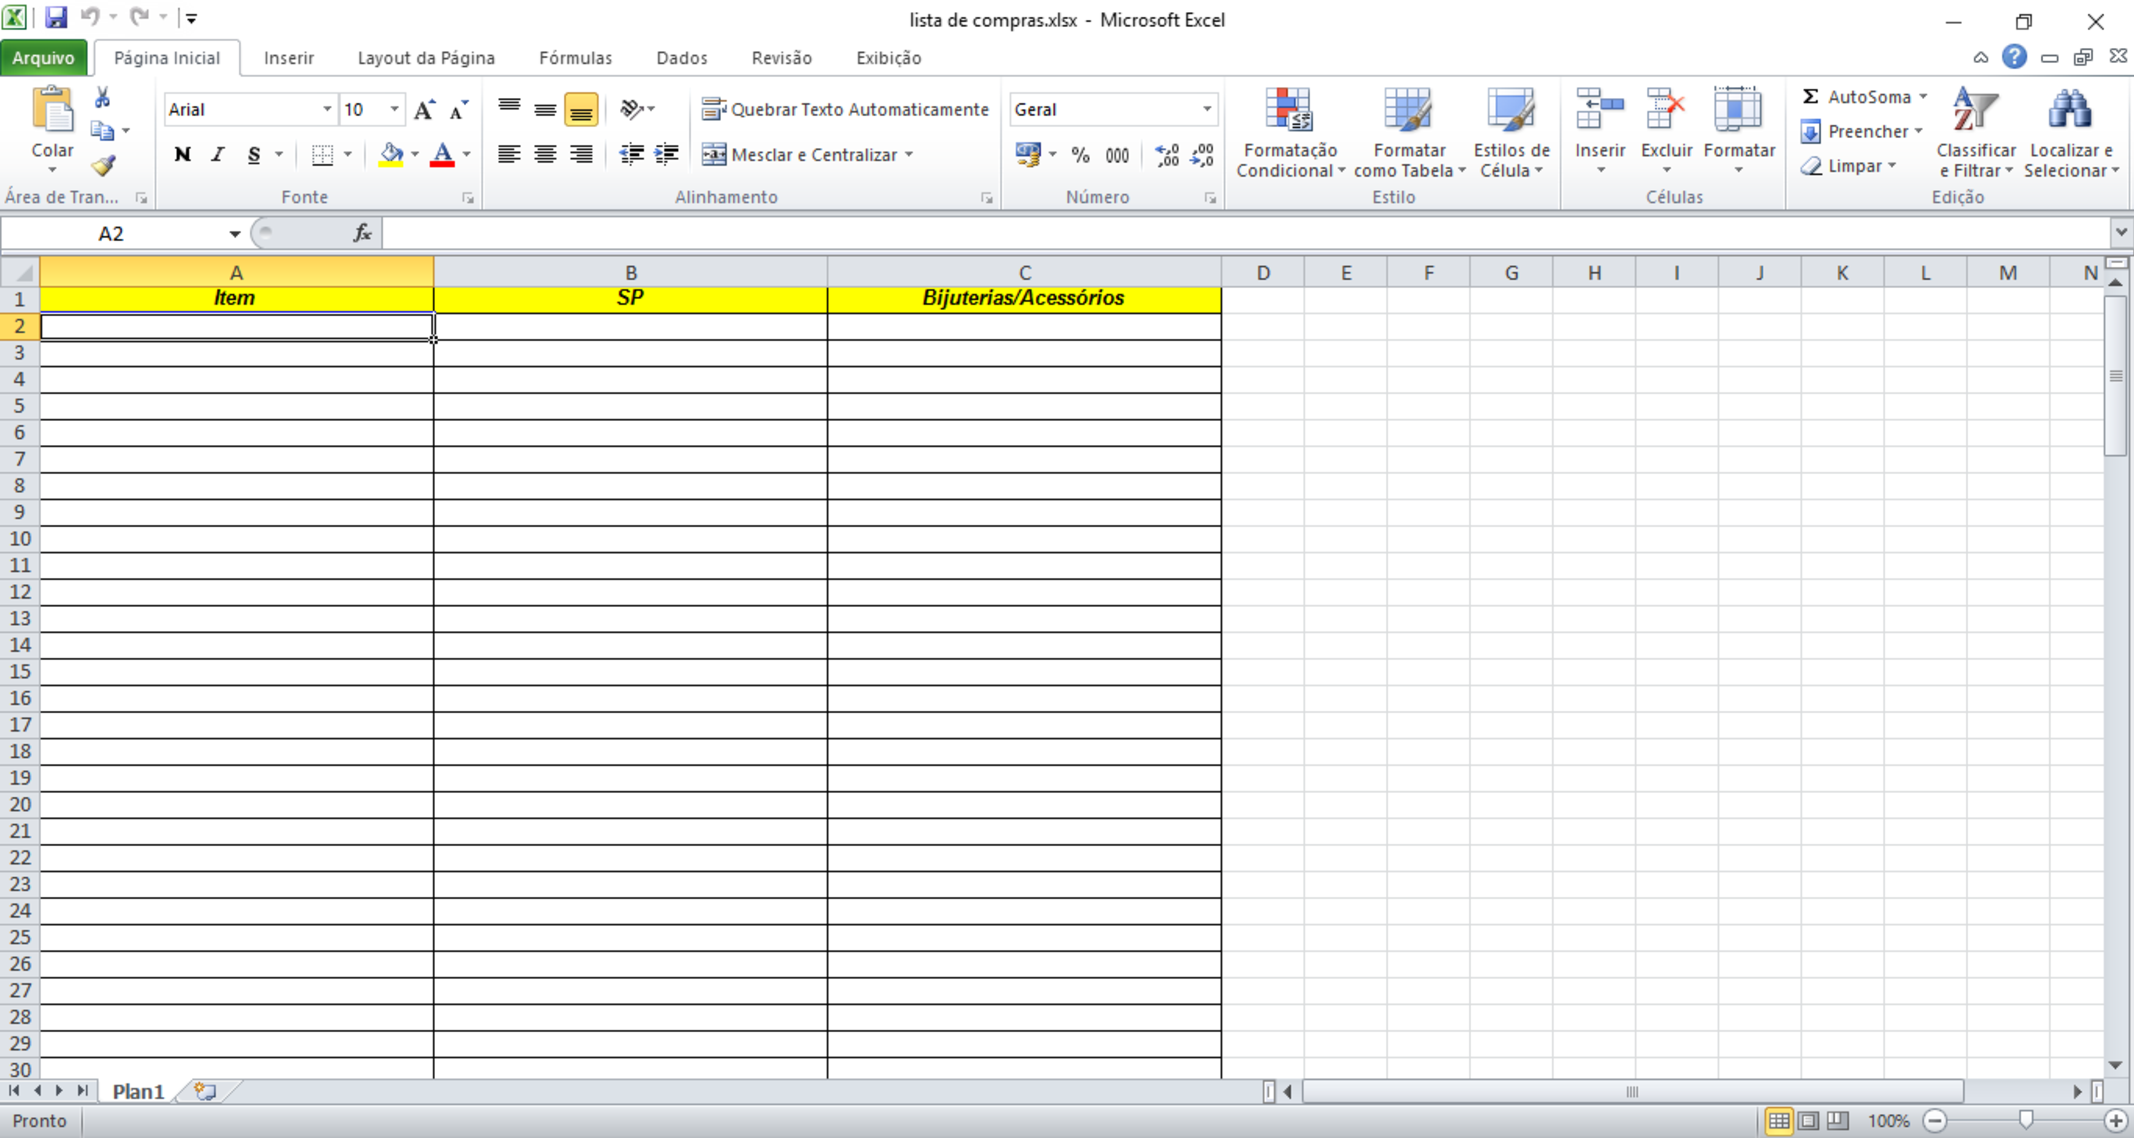
\includegraphics[width=.9\textwidth,keepaspectratio]{figures/lista-excel.pdf}
\caption{Planilha utilizada}
\label{fig:planilha}
\end{figure}

O costumeiro é que cada funcionária tenha sempre consigo uma caderneta (no bolso do colete fornecido pela loja) e anote itens que são de sua seção assim que seja percebida a necessidade. Entende-se como necessidade: (\textit{i}) itens que ainda não sejam comercializados anteriormente, mas que um ou mais clientes demonstrem interesse e sejam pertinentes dentro da proposta de loja; (\textit{ii}) itens já comercializadas mas que tenham acabado ou estejam por acabar, bem como possa seu estoque não durar até a próxima compra.

Não é regra ou obrigatório anotar somente itens da seção a qual a funcionária é responsável, muito pelo contrário, prefere-se que seja assim pois antes ``pecar'' pelo excesso que pela falta, será pior um item não ter sido anotado do que estar repetido em listas diferentes. Pois na próxima etapa deve o digitador filtrar para que não permaneça itens duplicados, porém essa ação tem complicação por itens com nomes dúbios (descritos com termos diferentes) ou mesmo quando compostos por várias palavras podem estar em várias ordens ou abreviações. Quando no processo de compras esta lista é levada impressa conforme Figura \ref{fig:impressao}.

\begin{figure}[ht]
\centering
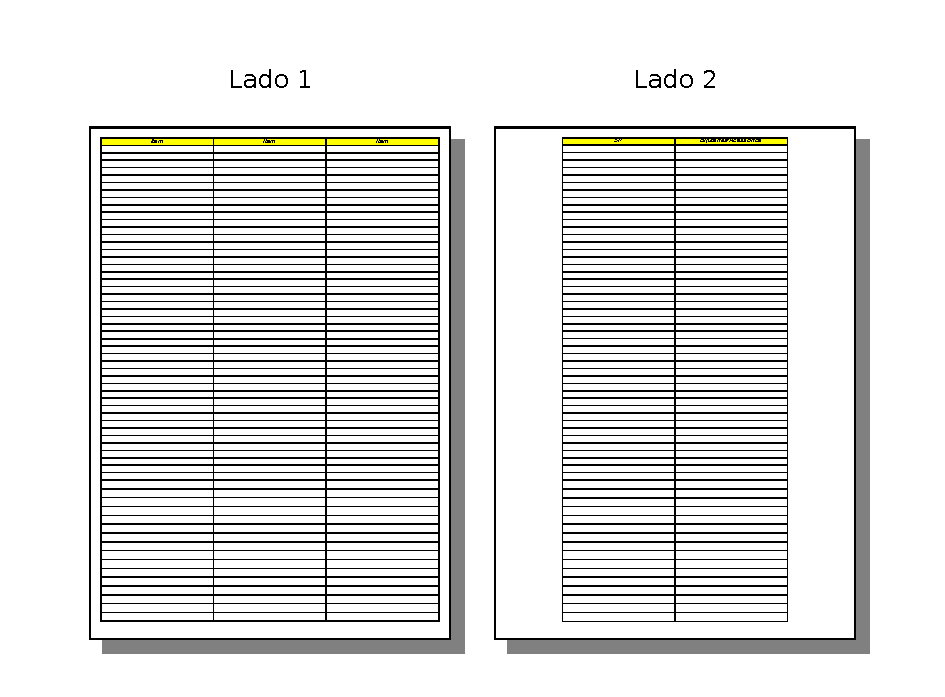
\includegraphics[width=.9\textwidth,keepaspectratio]{figures/modelo-impressao.pdf}
\caption{Modelo de Impressão da Planilha}
\label{fig:impressao}
\end{figure}

\section{Solução Proposta}

O sistema é uma aplicação para gerenciar os itens de compras, onde o usuário pode gerir listas (adicionar, editar ou remover itens), além de ser possível por usuários atribuídos marcar itens como comprados ou encerrar as listas. O acesso deverá ter algum processo de autenticação de usuário

Como explicado por \cite{sommerville2011}, a \textbf{Engenharia de Requisitos} é o processo em que são acordados e especificados os detalhes que satisfazem os envolvidos. Há dois níveis de detalhamento dessa especificação, um para clientes e usuários outro aos desenvolvedores, alto nível e abrangente respectivamente.

Os \textbf{Requisitos Funcionais} descrevem o que deve fazer o sistema, normalmente são descritos de modo abstrato para a fácil compreensão por seus usuários \cite{sommerville2011}. Puderam para o \textit{software} ser levantados os requisitos funcionais que seguem:
\begin{enumerate}
\item $[$RF001$]$ Realizar a adição de itens;
\item $[$RF002$]$ Manter as listas de itens;
\item $[$RF003$]$ Alternar o \textit{status} de compra dos itens;
\item $[$RF004$]$ Realizar encerramento das listas (manter itens não comprados);
\item $[$RF005$]$ Realizar autenticação para permitir o acesso.
\end{enumerate}

Já os \textbf{Requisitos Não funcionais} segundo \cite{sommerville2011}, são os relacionados não diretamente as funcionalidades oferecidas aos usuários pelo sistema. Descrevem esse requisitos como: confiabilidade, desempenho, proteção ou disponibilidade.
Foram definidos para o \textit{software}  os requisitos não funcionais à seguir:
\begin{enumerate}
\item $[$RNF001$]$ Acessível por navegadores, inclusive \textit{mobile};
\item $[$RNF002$]$ Interface intuitiva e minimalista;
\item $[$RNF003$]$ Tratamento em uso desconectado.
\end{enumerate}

Foram desenvolvidos os principais Diagramas UML, inicialmente o \textbf{Diagrama de Casos de Uso} (ver Figura \ref{fig:usecase}). Esse diagrama de acordo com \cite{guedes2011} este é o mais geral da UML, seu modo informal faz ser um dos primeiros a ser utilizado no levantamento e definição de requisitos. Costuma ser consultado também durante o processo, inclusive base para outros diagramas. Colabora ainda para que os usuários tenham ideia geral do funcionamento proposto, por sua simplicidade e fácil compreensão. Nesse diagrama são identificados atores (pessoas, sistemas, hardware) e funcionalidades, nele denominadas casos de uso.

\begin{figure}[ht]
\centering
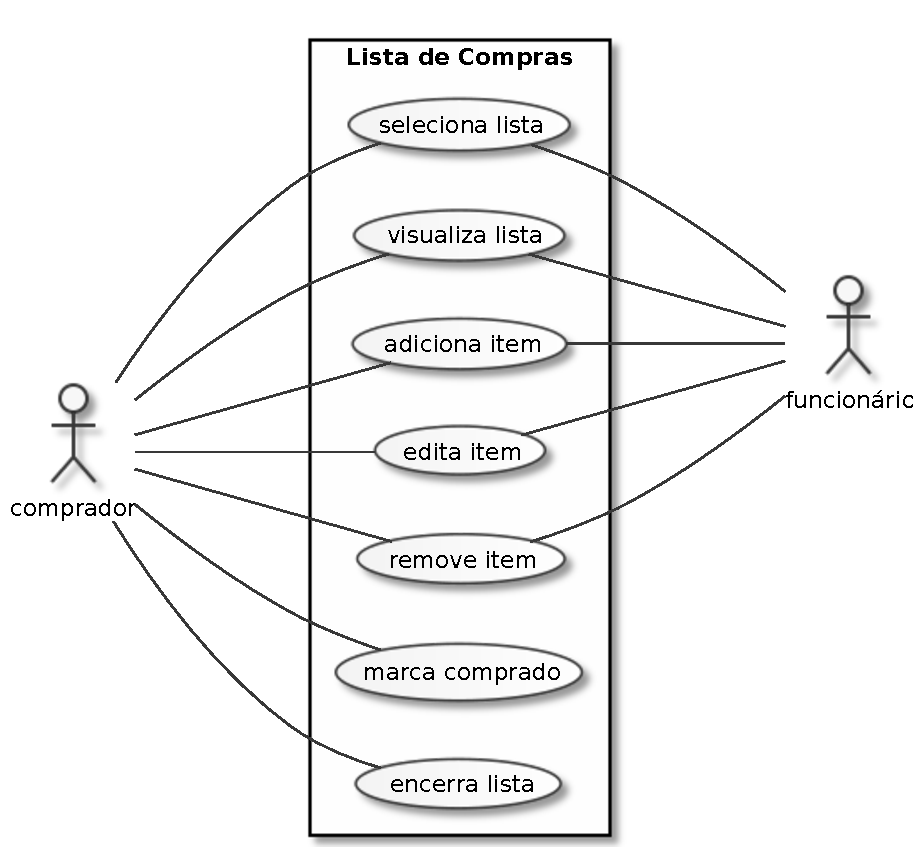
\includegraphics[width=.65\textwidth,keepaspectratio]{figures/usecase.pdf}
\caption{Diagrama de Casos de Uso}
\label{fig:usecase}
\end{figure}

Também foi criado o \textbf{Diagrama de Classes} (ver Figura \ref{fig:classes}) que é possivelmente o mais utilizado, além de importante é apoio para alguns dos demais diagramas \cite{guedes2011}. Este diagrama apresenta atributos, métodos e estrutura das classes, além da comunicação e relação entre elas.

\begin{figure}[ht]
\centering
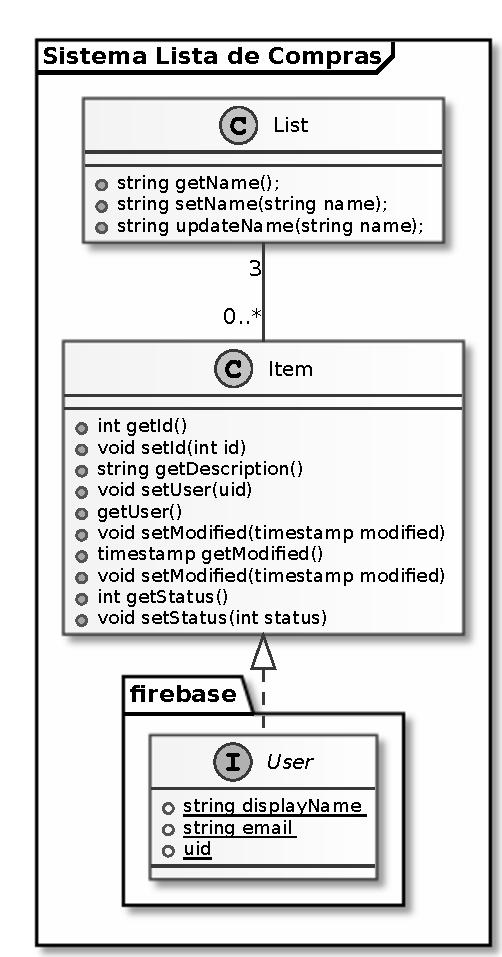
\includegraphics[width=.48\textwidth,keepaspectratio]{figures/classes.pdf}
\caption{Diagrama de Classes}
\label{fig:classes}
\end{figure}

A modelagem conceitual de banco de dados é descrita por \cite{heuser2009} como primeira etapa do projeto de banco de dados, seu objetivo é obter descrição abstrata dos dados, independente da implementação computacional que for realizada. A técnica mais difundida utiliza o modelo entidade-relacionamento (modelo ER), sua representação gráfica utiliza diagrama próprio (ver Figura \ref{fig:me}).

\begin{figure}[ht]
\centering
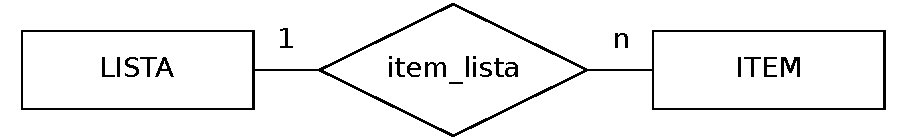
\includegraphics[width=.7\textwidth,keepaspectratio]{figures/mer.pdf}
\caption{Diagrama Entidade-Relacionamento}
\label{fig:me}
\end{figure}

\section{Acesso \textit{Offline}}

Com auxílio de \textbf{\textit{Service Workers}} (SW) é possível resolver a navegação \textit{offline}. Está sendo desenvolvido, como explica \cite{swfirstdraft}, por um esforço colaborativo entre grandes empresas como Google, Mozilla e outras. Sua implementação tem sido constante principalmente nos navegadores Chrome e Firefox. Realmente excitante para os interessados na competição entre web e aplicações nativas nos sistemas operacionais.

Sua implementação no modo mais básico em uma aplicação de página única pode ser considerada simples. Porém sua versatilidade e aplicabilidade é incrivelmente mais extensa. Inicialmente é necessário informar ao navegar o arquivo JavaScript, que será o controlador se comportando como se fosse um proxy local. Para isso utiliza-se o comando de registro (conforme Figura \ref{fig:swregister}), após testar se o navegador é compatível.

\begin{figure}[ht]
\centering
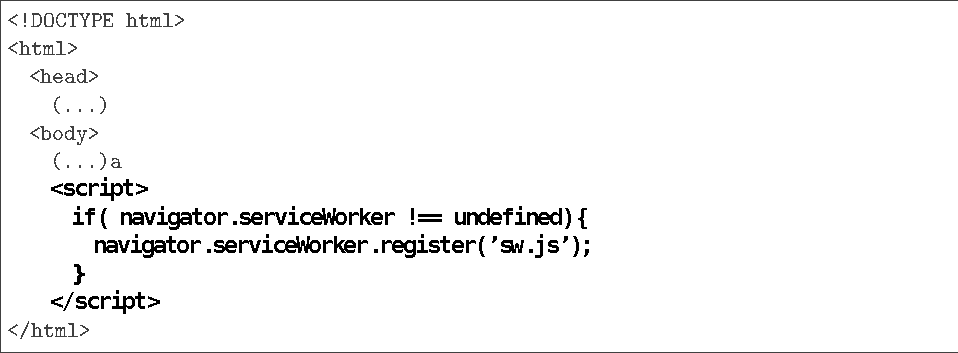
\includegraphics[width=.85\textwidth,keepaspectratio]{figures/html.pdf}
\caption{HTML destacando o registro do SW}
\label{fig:swregister}
\end{figure}

Dentro do arquivo \texttt{sw.js} (notável em Figura \ref{fig:swjs}) constam dois eventos: um de instalação, para quando o navegador de acordo com o registro instala (\textbf{\textit{install}}) e outro para captura de ação de rede (\textbf{\textit{fetch}}), onde iria naturalmente requisitar determinado recurso. O evento de instalação lista os arquivos a serem armazenados e no de rede indica a utilização dos arquivos armazenados.

\begin{figure}[ht]
\centering
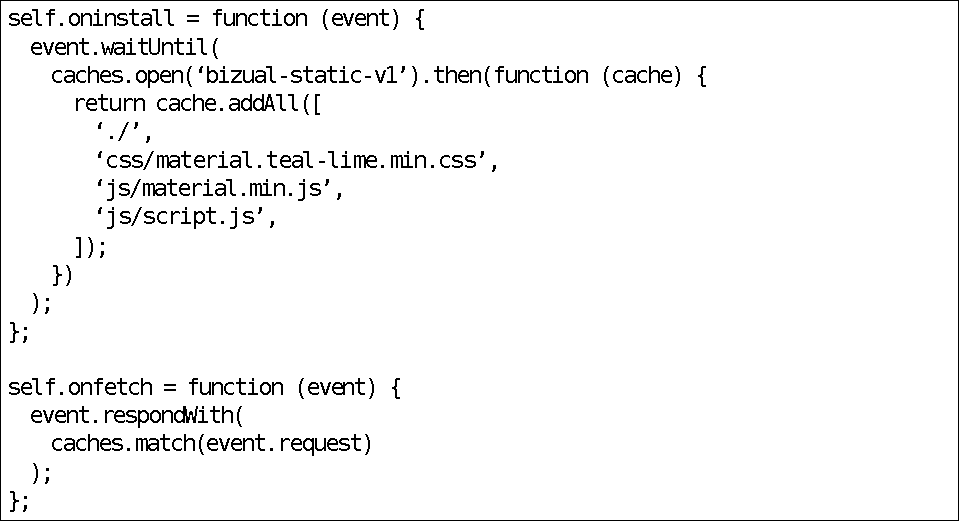
\includegraphics[width=.85\textwidth,keepaspectratio]{figures/sw.pdf}
\caption{Conteúdo do arquivo SW}
\label{fig:swjs}
\end{figure}

Durante o artigo foi utilizada a denominação ``navegador moderno'' neste estudo são navegadores que apostam em novas tecnologia que estejam surgindo. Normalmente podem ser considerados o Google Chrome, Mozilla Firefox e Opera. A Microsoft vêm flexibilizando essas adoções nas últimas versões e do seu subistituto o Edge, porém quando tecnologias ainda em rascunho ela opta por sua definição e maturidade. A Tabela \ref{tab:swcompatibility} apresenta como está, mesmo que parcial, essa compatibilidade. Ressaltando o quão recente é essa adoção, as versões lançadas somente neste ano como estáveis entre 9 de setembro e 23 de outubro, são nesses navegadores a primeira implementação ocorrida. Apenas o Google Chrome para desktop possui compabilidade nas versões anteriores, desde 2 de maio também deste ano.

\begin{table}[ht]
\centering
\begin{tabular}{ C{46pt} | C{46pt} | C{46pt} | C{46pt} | C{46pt} | C{46pt} | C{46pt} }\hline
Edge & Firefox & Chrome & Safari & Opera & iOS & Android \\ \hline
 & 49+ & 49+ &  & 41+ &  & 5.0+ \\ \hline
\end{tabular}
\caption{Suporte à SW pelos navegadores}
\label{tab:swcompatibility}
\end{table}

\section{Considerações Finais}

A resistência em automatização em pequenos comércios é uma realidade. Nem em situações em que o custo é mínimo e as vantagens são evidentemente mensuradas há o apoio necessário.
Foi documentada uma proposta para definição de um domínio na internet e contratação do serviço de hospedagem, que devido a outras prioridades não foi devidamente apreciado. Devido a esta falta de aprovação foi aqui considerado como negado, pelo menos para o período de início e fim do presente estágio.

%O projeto foi inicialmente acordado verbalmente com boa aceitação. Após o listado como solução proposta, continuou o aceite porém com ressalvas. A principal diz respeito a uso de smartphone ser levemente controlado, por solicitação quando possível deixar em seu armário ou com uso muito restrito, apenas para que não haja um abuso. Outra ressalva, em continuidade à anterior, são as poucas funcionárias que por opção não se utilizam de celulares, devendo assim ser possível selecionar qual funcionário através de alguns logins.

Foi atingido o essencial que era o estudo do caso e o estudo de viabilidade, bem como levantamento, requisitos, diagramas, banco de dados.
Houve atraso tecnológico devido ao investimento necessário em serviço de hospedagem do servidor. Ficando a própria implementação da solução como trabalho futuro.

%Como trabalho futuro fica o desenvolvimento e implementação da solução proposta. O supervisor sugeriu acrescentar a possibilidade de informar o valor da compra para consulta em compras posteriores para comparativo.

%Também foi notado pelo supervisor que não há smartphones corporativos e nem todos os funcionários têm aparelhos para o uso proposto, logo deve possibilitar a troca após logado de qual funcionário está informando o item. Foi sugerido e é possível que no próximo ano o celular corporativo deixe de ser um feature phone para ser um smartphone.

\bibliographystyle{sbc}
\bibliography{references}

\includepdf[pages=-]{report.pdf}
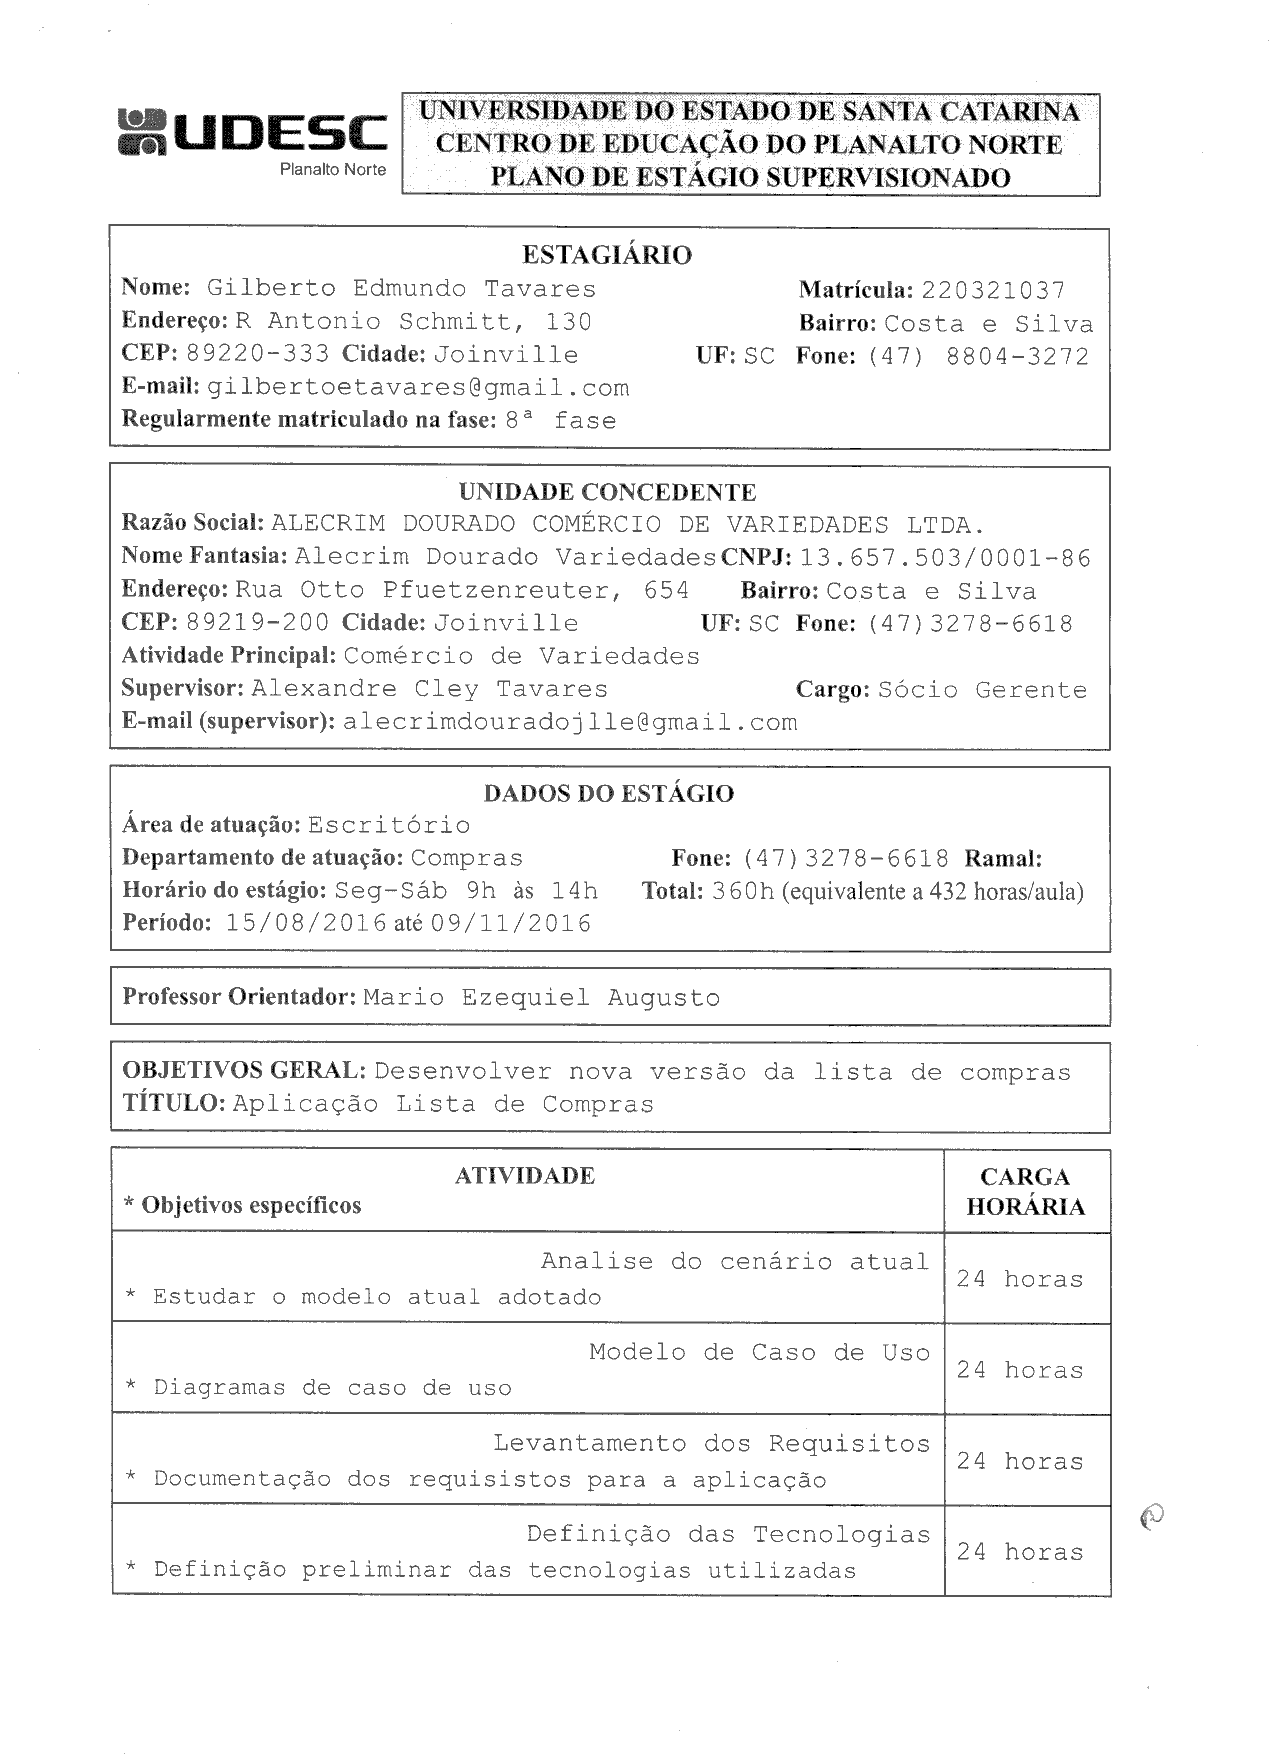
\includepdf[pages=-]{scanned/plano.pdf}
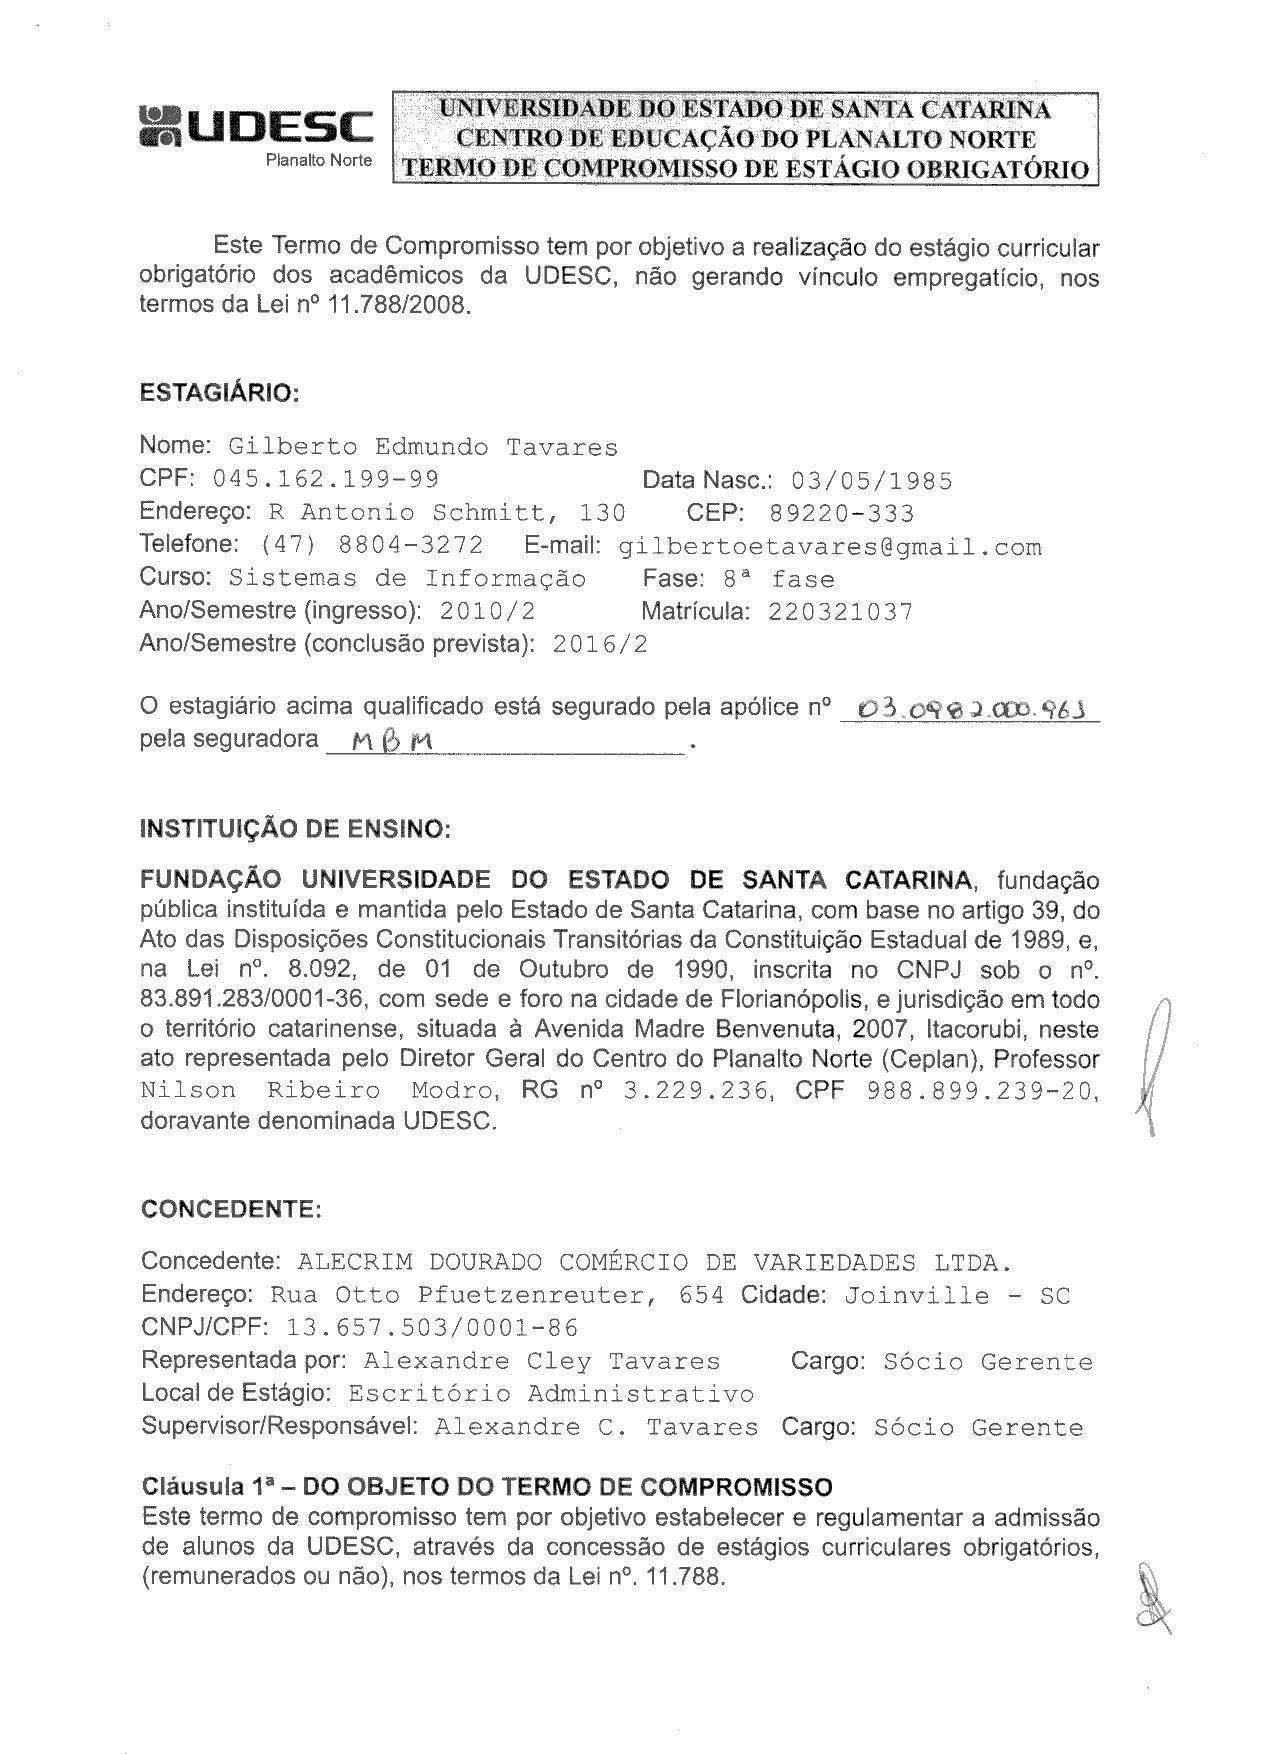
\includepdf[pages=-]{scanned/termo.pdf}
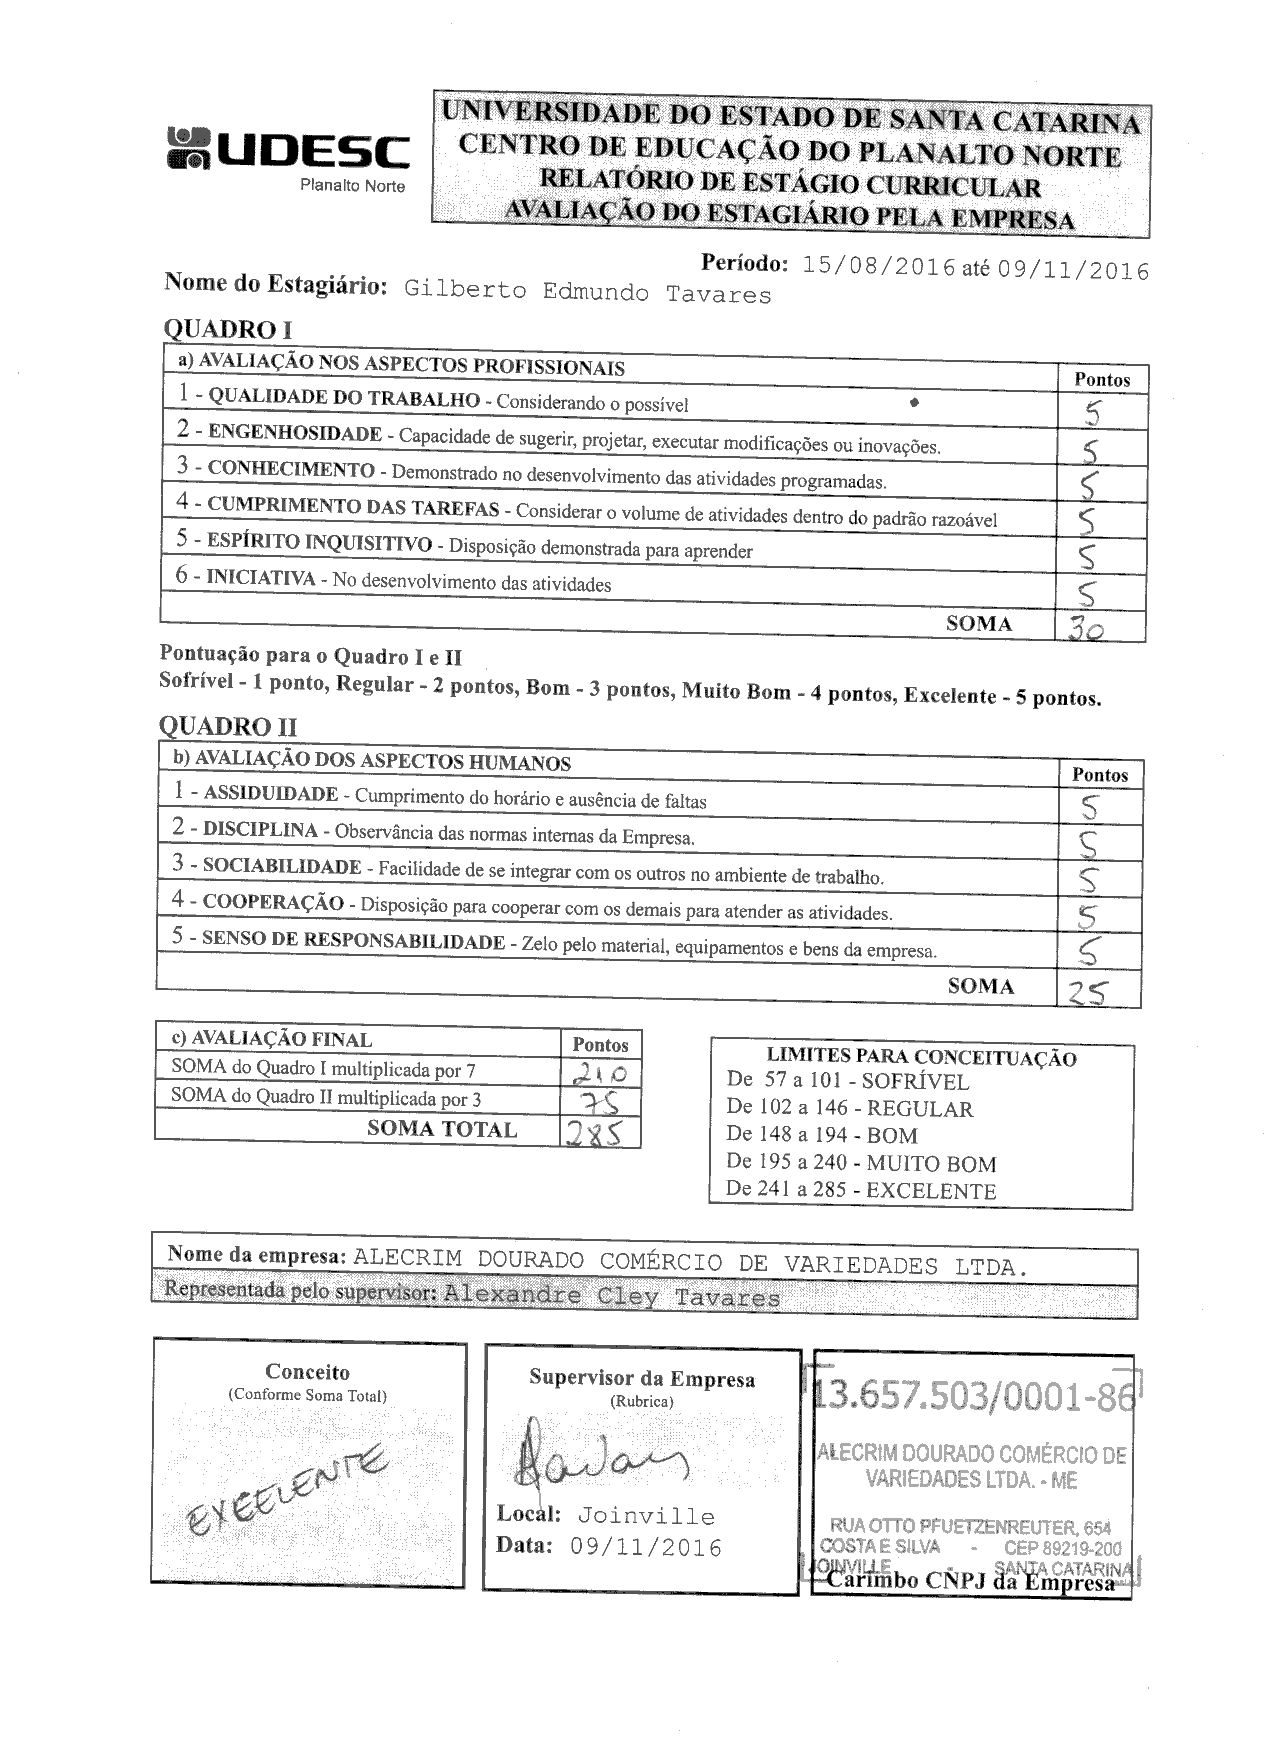
\includepdf{scanned/supervisor.pdf}
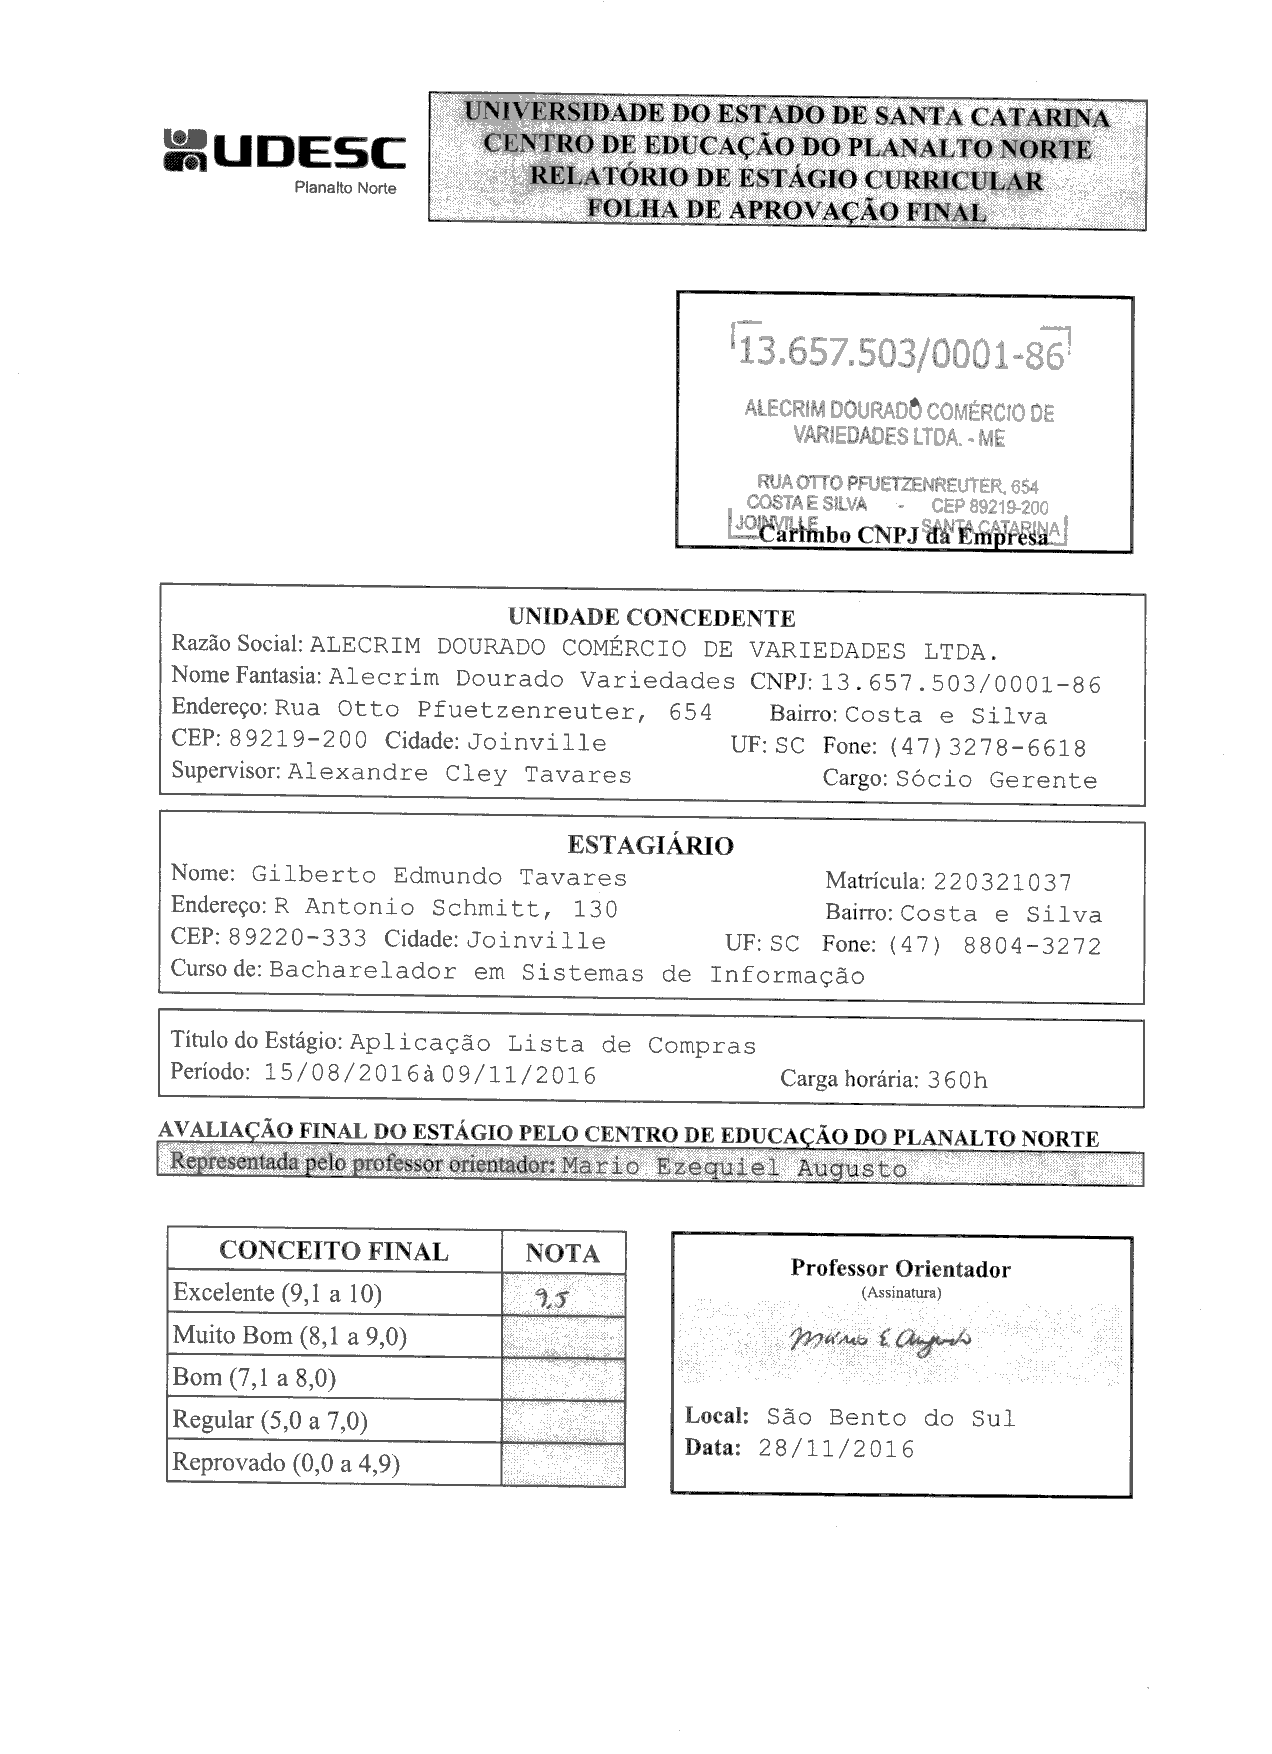
\includepdf{scanned/orientador.pdf}

\end{document}
